\documentclass[10pt]{beamer}

% 1. Theme and Sidebar Setup
\usetheme{Hannover}
\usecolortheme{dolphin}

% 2. Custom Light Blue Color Palette
\definecolor{lightskyblue}{RGB}{235, 248, 255}
\definecolor{navyblue}{RGB}{3, 105, 161}
\definecolor{borderblue}{RGB}{186, 230, 253}

\setbeamercolor{sidebar}{bg=lightskyblue, fg=navyblue}
\setbeamercolor{section in sidebar}{fg=navyblue}
\setbeamercolor{titlelike}{fg=navyblue}
\setbeamercolor{structure}{fg=navyblue}
\setbeamercolor{block title}{bg=borderblue, fg=navyblue}
\setbeamercolor{block body}{bg=lightskyblue!50, fg=black}

% Apply smaller font globally to blocks to prevent overflow
\setbeamerfont{block body}{size=\small}
\setbeamerfont{block title}{size=\small}

\usepackage{tikz}
\usepackage{amsmath}

\begin{document}

% --- SECTION 1: EXAMPLE 1A ---
\section{Example 1a}
\begin{frame}{Example 1a: Find $x$}
    \begin{columns}[T] % T for top alignment
        \begin{column}{0.65\textwidth}
            \begin{block}{Step-by-Step Solution}
                \begin{enumerate}
                    \item<1-> \textbf{Identify Triangle Type:} \\
                    $90^\circ - 45^\circ = 45^\circ$. \\
                    This is a 45$^\circ$-45$^\circ$-90$^\circ$ triangle.
                    
                    \item<2-> \textbf{Relationship:} \\
                    $\text{Hypotenuse} = \text{Leg} \cdot \sqrt{2}$
                    
                    \item<3-> \textbf{Substitute and Solve:} \\
                    $\text{Leg} = 6$ \\
                    $x = 6\sqrt{2}$
                \end{enumerate}
            \end{block}
        \end{column}

        \begin{column}{0.35\textwidth}
            \centering
            \vspace{0.2cm}
            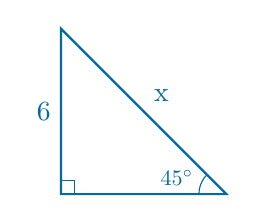
\begin{tikzpicture}[scale=0.7]
                \coordinate (A) at (0,3);
                \coordinate (B) at (0,0);
                \coordinate (C) at (3,0);
                \draw[thick, navyblue] (A) -- (B) node[midway, left] {6} -- (C) -- cycle node[midway, above right] {x};
                \draw[navyblue] (0,0.25) -- (0.25,0.25) -- (0.25,0);
                \draw[navyblue] (2.5,0) arc (180:135:0.5);
                \node[navyblue, scale=0.8] at (2.1,0.3) {45$^\circ$};
            \end{tikzpicture}
        \end{column}
    \end{columns}
\end{frame}

% --- SECTION 2: EXAMPLE 1B ---
\section{Example 1b}
\begin{frame}{Example 1b: Find $x$}
    \begin{columns}[T]
        \begin{column}{0.65\textwidth}
            \begin{block}{Step-by-Step Solution}
                \addtolength{\itemsep}{-0.5ex} % Tighten vertical list spacing
                \begin{enumerate}
                    \item<1-> \textbf{Identify Triangle Type:} \\
                    Legs are congruent ($\text{Leg} = 9\sqrt{2}$). \\
                    It is a 45$^\circ$-45$^\circ$-90$^\circ$ triangle.
                    
                    \item<2-> \textbf{Relationship:} \\
                    $\text{Hypotenuse} = \text{Leg} \cdot \sqrt{2}$
                    
                    \item<3-> \textbf{Substitute Value:} \\
                    $x = (9\sqrt{2}) \cdot \sqrt{2}$
                    
                    \item<4-> \textbf{Simplify Answer:} \\
                    $x = 9 \cdot (\sqrt{2} \cdot \sqrt{2})$ \\
                    $x = 9 \cdot 2 = 18$
                \end{enumerate}
            \end{block}
        \end{column}

        \begin{column}{0.35\textwidth}
            \centering
            \vspace{0.5cm}
            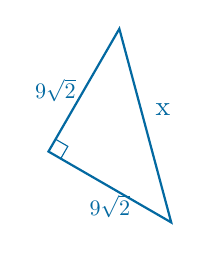
\begin{tikzpicture}[scale=0.6, rotate=-30]
                \coordinate (A) at (0,3);
                \coordinate (B) at (0,0);
                \coordinate (C) at (3,0);
                \draw[thick, navyblue] (A) -- (B) node[midway, left, scale=0.8] {$9\sqrt{2}$} -- (C) node[midway, below, scale=0.8] {$9\sqrt{2}$} -- cycle node[midway, above right] {x};
                \draw[navyblue] (0,0.3) -- (0.3,0.3) -- (0.3,0);
            \end{tikzpicture}
        \end{column}
    \end{columns}
\end{frame}

\end{document}